
\documentclass[mathserif]{beamer}
\usepackage{etoolbox}
% \usepackage{mathptmx}

\usecolortheme{beaver}
\definecolor{mygreen}{cmyk}{0.82,0.11,1,0.25}
\setbeamertemplate{blocks}[rounded][shadow=false]
\addtobeamertemplate{block begin}{\pgfsetfillopacity{0.8}}{\pgfsetfillopacity{1}}
\setbeamercolor{structure}{fg=mygreen}
\setbeamercolor*{block title example}{fg=blue!50,
bg= blue!10}
\setbeamercolor*{block body example}{fg= blue,
bg= blue!5}

\usepackage{ulem}
\usepackage{cancel}
\usefonttheme{professionalfonts}
{\vspace*{.10mm}}
\usetheme[height=10mm]{Rochester}
\title{ Lagoon Overflow Project}
\author{}
\date{}


\begin{document}
\maketitle

\begin{frame}
 \frametitle{Introdution}
{\vspace*{.010mm}}

\begin{figure}[httb!]
\centering
  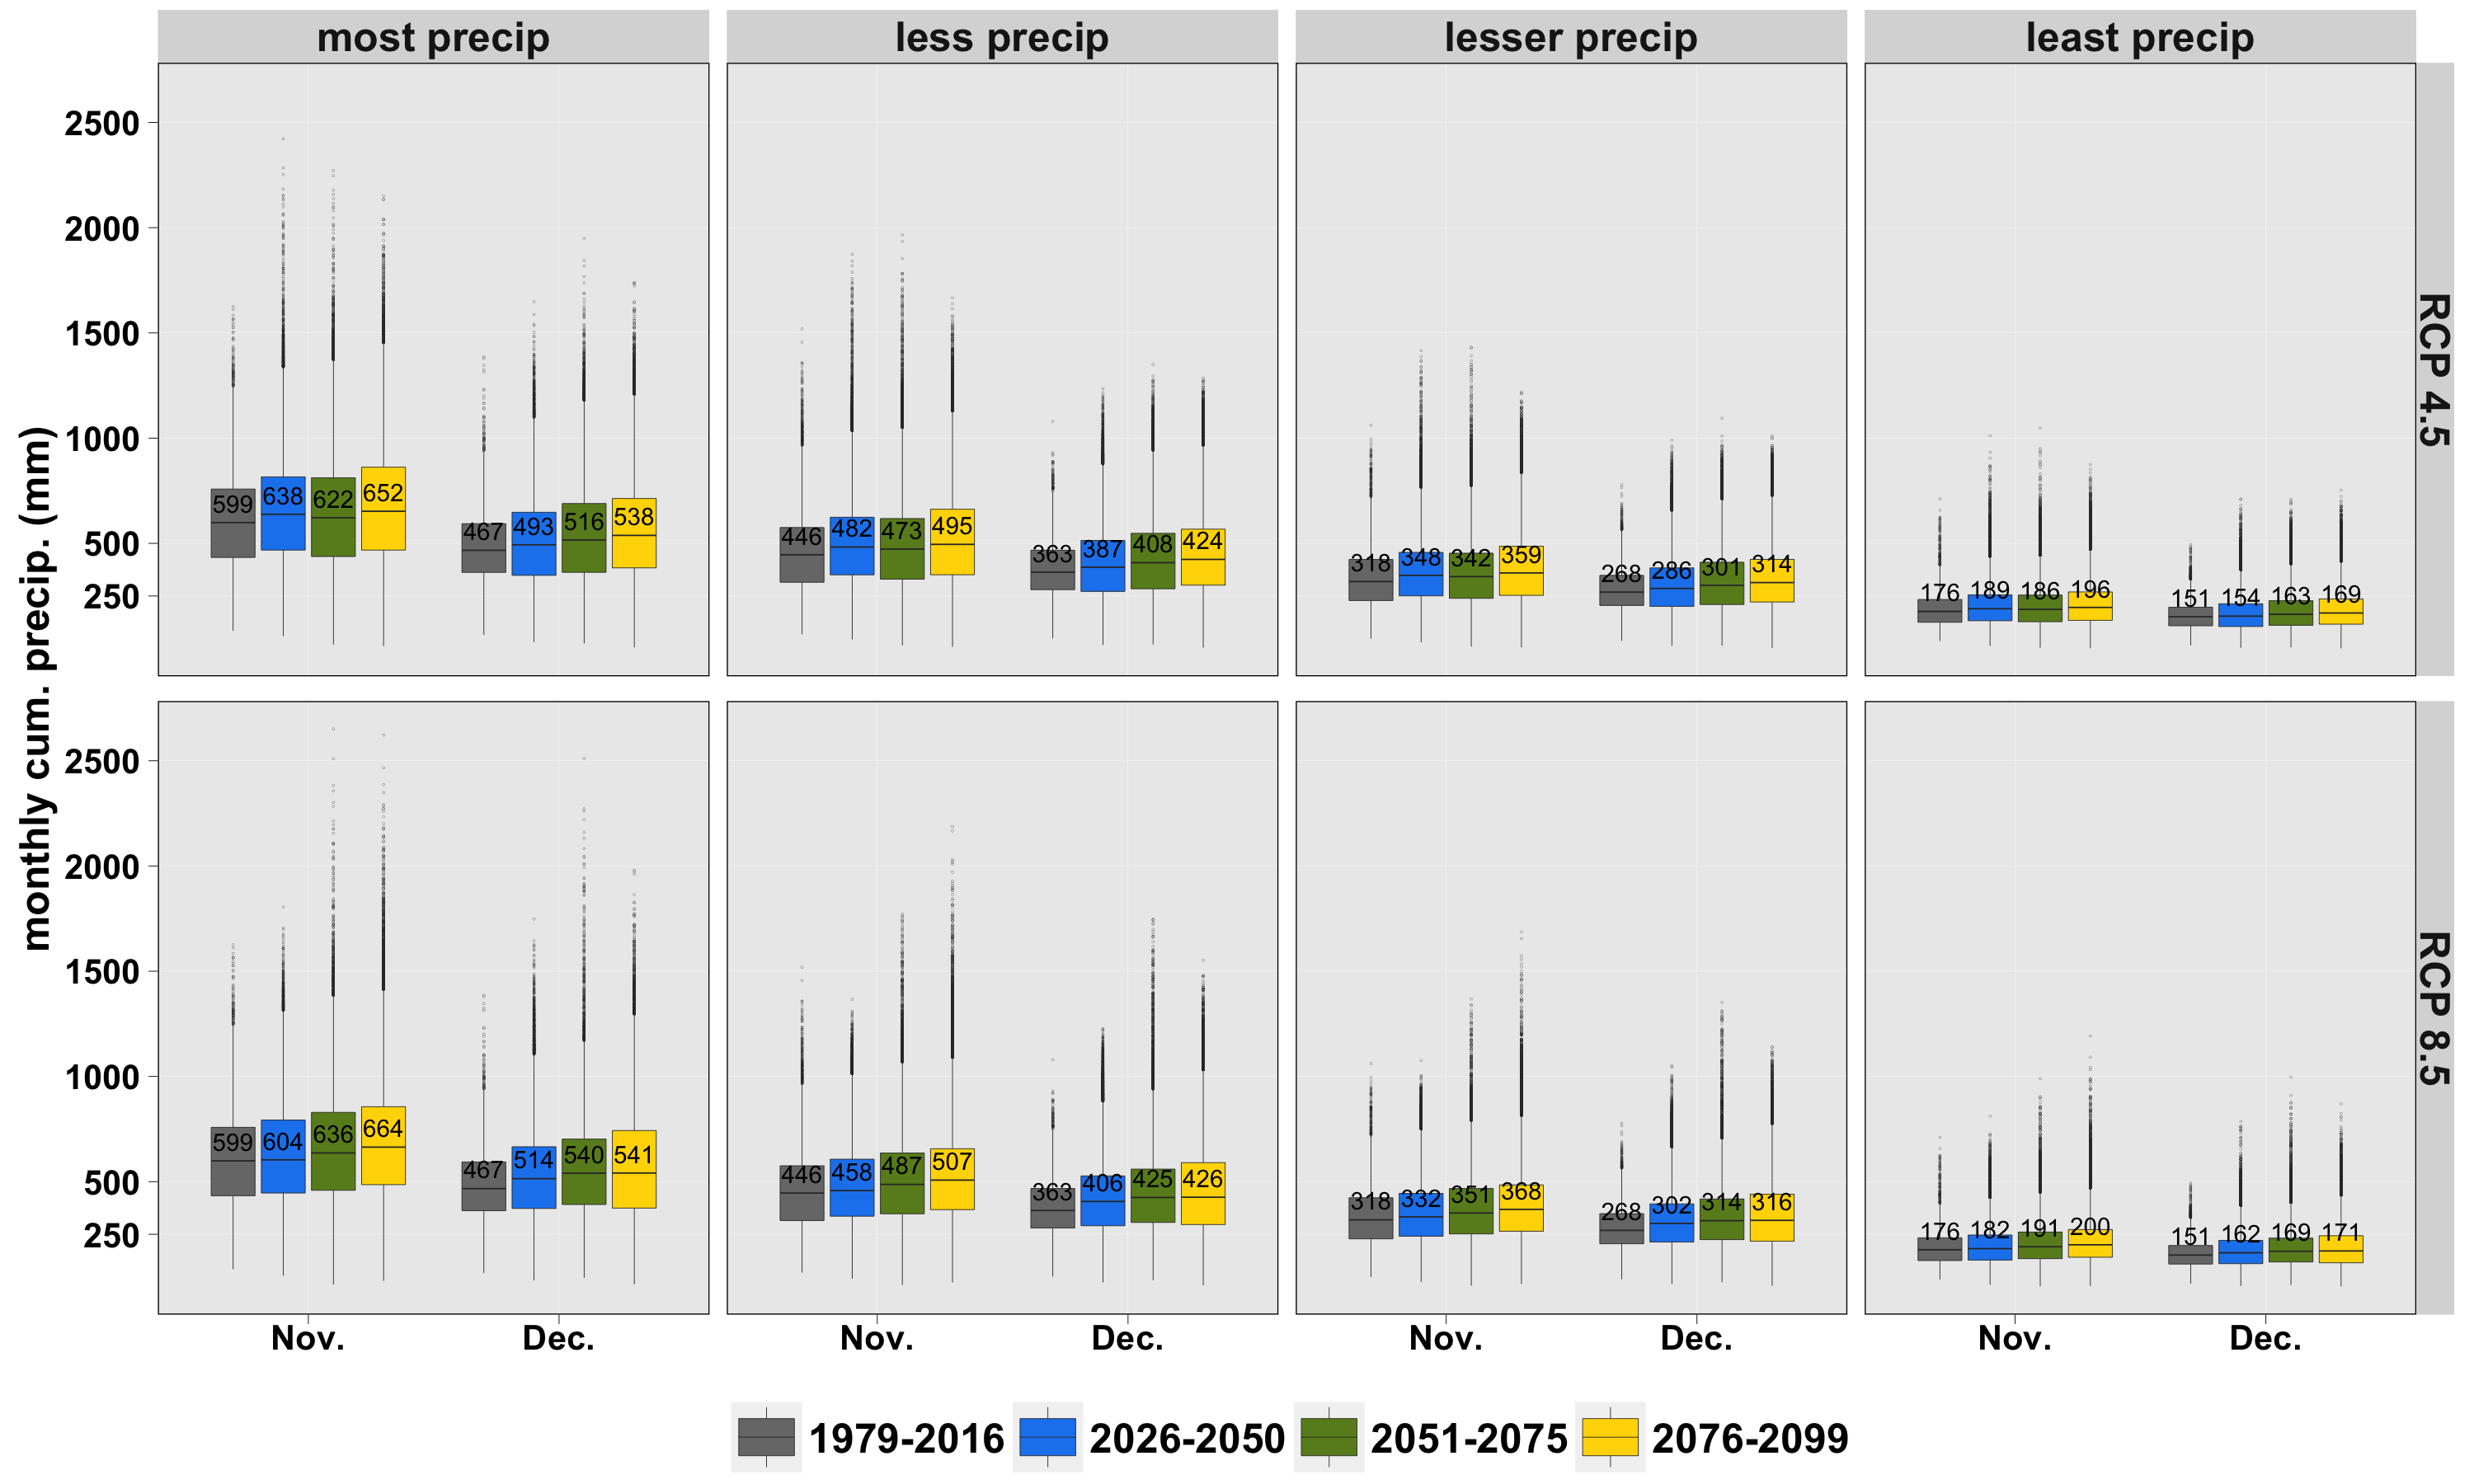
\includegraphics[width=1\linewidth]{figures/nov_Dec_box}
\end{figure}
\end{frame}


\begin{frame}
 \frametitle{Introdution}
\begin{itemize}[<+->]

\item Note that $p_n(z)=1-zq_{n-1}(z)$ and therefore, $p_n(0)=1.$

\end{itemize}
\end{frame}


\begin{frame}
 \frametitle{IDR for Solving Linear Systems}
\textbf{IDR} is a Krylov subspace solver with one more flavor. The residuals in IDR are forced to be in subspaces $\mathcal{G}_j$ of decreasing dimension.\pause
These nested subspaces are defined by: \begin{center}$\mathcal{G}_j=(\mathbf{I}-\omega_j\mathbf{A})(\mathcal{G}_{j-1} \cap \mathcal{S})$\end{center}
where $\mathcal{S}$ is a fixed proper subspace of $\mathbb{C}^N$ and $0 \ne \omega_j$'s are scalars.\\
\pause
\vspace{.1in}
\begin{theorem}
Let $\mathbf{A}$ be any matrix in $\mathbb{C}^{N \times N}$ and let $v\ne 0$ be any vector in $\mathbb{C}^N$, and let  $\mathcal{G}_0$ be the full Krylov space $\mathcal{K}_{N+1}(\mathbf{A},\mathbf{v})$. Let $\mathcal{S}$ be any (proper) subspace of $\mathbb{C}^N$ such that $\mathcal{G}_0$ and $\mathcal{S}$ do not share any nontrivial invariant subspace of $\mathbf{A}$ and define $\mathcal{G}_j$ by

\begin{center} $ \mathcal{G}_j=(\mathbf{I}-\omega_j\mathbf{A})(\mathcal{G}_{j-1} \cap \mathcal{S})$  \end{center}

for $j=1, 2, 3, \cdots$ where $0\ne \omega_j$ are scalars then:\\
\pause
$(i)$ $\mathcal{G}_j \subset \mathcal{G}_{j-1}$, $\forall j> 0.$\\
\pause
$(ii)$ $\mathcal{G}_j=\{\mathbf{0}\}$ for some $j \le N$\\
\vspace{.1in}

\end{theorem}
\end{frame}

\begin{frame}
\frametitle{Derivation of IDR Algorithm}

Usually in Krylov solvers we find $\mathbf{x}_n$ then we find corresponding $\mathbf{r}_n$. In IDR we will do the other way arround, if a recurssion for $\mathbf{r}_n$'s is given, we have to be able to find corresponding $\mathbf{x}_n$'s. \pause Assuming this is possible we have the following, Let $\nabla u_k:=u_k-u_{k-1}.$\\


\vspace{.1in}
$\begin{array} {lclcl} \mathbf{A}\nabla \mathbf{x}_{n+1}=\mathbf{A}(\mathbf{x}_{n+1}-\mathbf{x}_n)  & = & \mathbf{A}\mathbf{x}_{n+1} \hspace{.3in} -\mathbf{A}\mathbf{x}_n \\ & = & \mathbf{A}\mathbf{x}_{n+1}-\mathbf{b}+\mathbf{b} -\mathbf{A}\mathbf{x}_n \\&=& \vspace{.1in} -\mathbf{r}_{n+1}+\mathbf{r}_n \\&=& \vspace{.1in} -p_{n+1}(\mathbf{A})\mathbf{r}_0+p_n(\mathbf{A})\mathbf{r}_0 \\&=& \vspace{.1in} (p_n(\mathbf{A})-p_{n+1}(\mathbf{A}))\mathbf{r}_0\end{array}$


\pause
We can find $\mathbf{x}_{n+1}$ here without solving the system if $p_n(z)-p_{n+1}(z)$ is divisible by $z$, as follows:

\pause
\begin{center}
$ \textcolor{red}{\cancel{\textcolor{black}{\mathbf{A}}}} \nabla \mathbf{x}_{n+1} = \textcolor{red}{\cancel{\textcolor{black}{\mathbf{A}}}} \psi_n(\mathbf{A})\mathbf{r}_0 $

\end{center}

\end{frame}

\begin{frame}
\frametitle{Derivation of IDR Algorithm}

We saw in any Krylov solvers $\mathbf{r}_n=p_n(\mathbf{A})\mathbf{r}_0 \in \mathcal{K}_{n+1}(\textcolor{red} {\backslash \mathcal{K}_n})$ where degree of $p_n$ is exactly $\textcolor{red}{n}$. 
\pause
Therefore, we have:\\

\begin{center} $\mathbf{r}_n=\textstyle{\sum\limits _{k=0}^{n}} \alpha_k \mathbf{A}^{k}\mathbf{r}_0$ , $\alpha_n \ne 0$ \end{center}

\pause
\mbox{Let $\mathbf{v}_n \in \mathcal{K}_{n+1} \backslash \mathcal{K}_n$ be any arbitrary vector, then $\mathbf{A}\mathbf{v}_n \in \mathcal{K}_{n+2} \backslash \mathcal{K}_{n+1}$}.\\

\pause
Hence, any arbitrary vector in $\mathcal{K}_{n+2} \backslash \mathcal{K}_{n+1}$ can be written as:

\[ -\alpha \mathbf{A}\mathbf{v}_n+\sum\limits_{k=0}^{n} \beta_k \mathbf{r}_{n-k}  \]

\pause
Therefore, we can write:  \[\mathbf{r}_{n+1}=-\alpha \mathbf{A}\mathbf{v}_n+\sum\limits_{k=0}^{n} \beta_k \mathbf{r}_{n-k}\]
\end{frame}


\begin{frame}
\frametitle{Derivation of IDR Algorithm}
Our goal was computing $\mathbf{x}_{n+1}$ provided that $\mathbf{r}_{n+1}$ is known. Let's replace $r_i$'s by $\mathbf{b}-\mathbf{A}\mathbf{x}_i$ in above formula to get $\mathbf{x}_{n+1}$:

\pause
\[\mathbf{r}_{n+1}=-\alpha \mathbf{A}\mathbf{v}_n+\sum\limits_{k=0}^{n} \beta_k \mathbf{r}_{n-k} \textcolor{blue}{ \longrightarrow} \] 

\[\begin{array} {lclcl}  \mathbf{b}-\mathbf{A} \mathbf{x}_{n+1}&=& -\alpha \mathbf{A} \mathbf{v}_n + \sum_{k=0}^n \beta_k (\mathbf{b}-\mathbf{A} \mathbf{x}_{n-k})\nonumber \vspace{.1in} \\&=& (\sum \limits_{k=0}^n \beta_k)\mathbf{b}-\mathbf{A}(\alpha \mathbf{v}_n +\sum \limits_{k=0}^n \beta_k \mathbf{x}_{n-k})\end{array}\]

\pause
Consequently $\mathbf{x}_{n+1}$ would be solution of \[\mathbf{A} \mathbf{x}_{n+1} =(1- \sum_{k=0}^n \beta_k) \mathbf{b}+\mathbf{A}(\alpha \mathbf{v}_n+\sum_{k=0}^n \beta_k \mathbf{x}_{n-k}).\]

\pause
\mbox{$\mathbf{x}_{n+1}$ is computable without solving the system if $(1- \sum_{k=0}^n \beta_k)=0$.}
\end{frame}


\begin{frame}
\frametitle{Derivation of IDR Algorithm}
We want $1- \sum_{k=0}^n \beta_k=0$ or equivalently $ \sum_{k=0}^n \beta_k=1$. This equation can be established by:

\[\sum_{k=0}^n\beta_k \mathbf{r}_{n-k}=\mathbf{r}_n -\sum_{k=1}^n \gamma_k \nabla \mathbf{r}_{n-k+1}.\]

\pause
Because,

$\begin{array} {lclclcl}  \beta_0\mathbf{r}_n+\beta_1 \mathbf{r}_{n-1}+ \cdots +\beta_n\mathbf{r}_0 &=& \mathbf{r}_n-\gamma_1\nabla \mathbf{r}_n -\gamma_2 \nabla \mathbf{r}_{n-1} - \cdots \gamma_n\nabla \mathbf{r}_1 \\&=& (1-\gamma_1)\mathbf{r}_n+(\gamma_1-\gamma_2)\mathbf{r}_{n-1}+\cdots \\&& \hspace{.7in}+(\gamma_{n-1}-\gamma_n)r_1+\gamma_n\mathbf{r}_0  \end{array}$

\pause
which implies:

$\begin{array} {lclclcl}  
\beta_0&=&1-\textcolor{red}{\cancel{\textcolor{black}{\gamma_1}}}\\
\beta_1&=&\textcolor{red}{\cancel{\textcolor{black}{\gamma_1}}}-\textcolor{blue}{\cancel{\textcolor{black}{\gamma_2}}}\\
&\vdots&\\
\beta_n &=& \textcolor{green}{\cancel{\textcolor{black}{\gamma_1}}}
\end{array}$

\end{frame}

\begin{frame}
\frametitle{Derivation of IDR Algorithm}
So, in general for any Krylov solver we can write:
\[\mathbf{r}_{n+1}=-\alpha \mathbf{A}\mathbf{v}_n+\sum\limits_{k=0}^{n} \beta_k \mathbf{r}_{n-k}. \]

\pause
Now let's replace $\sum\limits_{k=0}^{n} \beta_k \mathbf{r}_{n-k} $ by $\mathbf{r}_n -\sum_{k=1}^n \gamma_k \nabla \mathbf{r}_{n-k+1}$ to get:

\begin{equation}\tag{2.1} \mathbf{r}_{n+1} =\mathbf{r}_n-\alpha \mathbf{A} \mathbf{v}_n-\sum \limits_ {k=1}^n \gamma_k \nabla \mathbf{r}_{n-k+1} \end{equation}

\pause
In equation (2.1) we are using all residuals from $0$ to $n$. Depth of recurssion is so long, in order to get short recurssions we need to have $\gamma_k=0$ for $k \ge m$ where $m \ll N$.\pause  So, I will change the upper limit from $n$ to $l$.
\end{frame}


\begin{frame}
\frametitle{Derivation of IDR Algorithm}
\begin{equation}\tag{2.2} \mathbf{r}_{n+1} =\mathbf{r}_n-\alpha \mathbf{A} \mathbf{v}_n-\sum \limits_ {k=1}^l \gamma_k \nabla \mathbf{r}_{n-k+1} \end{equation}
Equation (2.2) can be written in general for all Krylov solvers. It is time to add IDR flavor.\\
\pause

\vspace{.1in}We want to force residuals to be in $\mathcal{G}_{j+1}:=(\mathbf{I}-\omega_{j+1}\mathbf{A})(\mathcal{G}_{j}\cap \mathcal{S})$. 
Therefore, there should be a $\textcolor{red}{\mathbf{v}_n} \in \mathcal{G}_j\cap \mathcal{S}$ such that \begin{equation}\tag{2.3}\mathbf{r}_{n+1}=(\mathbf{I}-\omega_{j+1}\mathbf{A})\mathbf{v}_n\end{equation}


\pause
Equating (2.2) and (2.3) leads to \[\mathbf{v}_n := \mathbf{r}_n-\sum \limits_ {k=1}^l \gamma_k \nabla \mathbf{r}_{n-k+1} \hspace{.1in} \text{and}  \hspace{.1in} \alpha:=\omega_{j+1}\]  
\end{frame}


\begin{frame}
\frametitle{Derivation of IDR Algorithm}
Making this change in (2.2) gives the following:

\[\left\{ \tag{2.4}\begin{array}{llll} \mathbf{r}_{n+1} &=& (\mathbf{I}-\omega_{j+1} \mathbf{A}) \mathbf{v}_n\\ \mathbf{v}_n&=&\mathbf{r}_n-\sum \limits_ {k=1}^l \gamma_k \nabla \mathbf{r}_{n-k+1} \in \mathcal{G}_j\cap \mathcal{S}\end{array}\right.\]

\pause
Finding $\mathbf{v}_n$ and $\omega_j$ would be a great step toward our goal. So, let $\mathcal{S}:=\mathcal{N}(\mathbf{P}^*)$ where $\mathbf{P}=[\mathbf{p}_1 \hspace{.1in} \mathbf{p}_2 \hspace{.1in}  \cdots \hspace{.1in}  \mathbf{p}_s]$.  $\mathcal{S}$ has codimension $s$.
\vspace{.1in}

\pause
Since $\mathbf{v}_n \in \mathcal{S}$, we have to have $\mathbf{P}^*\mathbf{v}_n=0$, and consequently, \\
\[\mathbf{P}^*(\sum \limits_ {k=1}^l \gamma_k \nabla \mathbf{r}_{n-k+1}) =\mathbf{P}^*\mathbf{r}_n\]

\pause
\mbox{where $\gamma_k$'s are unknowns, so, we have a linear system of $s$ equations} in $l$ unknowns, which is uniquely solvable if $l=s.$
\end{frame}



\begin{frame}
\frametitle{Derivation of IDR Algorithm}
By letting $l=s$ and introducing the following new notaions equation (2.4) can be written in more compact form:
\pause
\vspace{.1in}
Let $\nabla \mathbf{R}_{n:n-s+1}:=[\nabla \mathbf{r}_n \hspace{.1in} \nabla \mathbf{r}_{n-1} \hspace{.1in}  \cdots \hspace{.1in} \nabla \mathbf{r}_{n-s+1}  ]$ and 

$\mathbf{c}_n=[\gamma_1 ^ {\textcolor{red}{{(n)}}} \hspace{.1in} \gamma_2 ^ {\textcolor{red}{{(n)}}} \cdots \gamma_s ^ {\textcolor{red}{{(n)}}}]^T$ gives the following:
\pause
\[\left\{ \tag{2.5}\begin{array}{llll} \mathbf{r}_{n+1} &=& (\mathbf{I}-\omega_{j+1} \mathbf{A}) \mathbf{v}_n\\ \mathbf{v}_n&=&\mathbf{r}_n-\nabla \mathbf{R}_{n:n-s+1}\mathbf{c}_n\end{array}\right.\]
\pause

For computing $\mathbf{v}_n$ we need $s+1$ residuals, therefore, computing the first residual in $\mathcal{G}_{j+1}$ needs $s+1$ residuals in $\mathcal{G}_j.$ So, we can expect $\mathbf{r}_{n+1}$ be in $\mathcal{G}_{j+1}$  if $n+1 \ge (j+1)(s+1)$. 

\pause
\vspace{.1in}
Therefore the relationship between $n$ and $j$ will be $j=\lfloor{\frac{n}{s+1}}\rfloor$.

\pause Since $\mathcal{G}_{j+1} \subset \mathcal{G}_j$ repeating these calculations will produce new residuals $r_{n+2}, r_{n+3},  \cdots$ in $\mathcal{G}_{j+1}.$
\end{frame}

\begin{frame}
\frametitle{Derivation of IDR Algorithm}
\textit{Choice of} $\omega_j$'s: The $\omega_{j+1}$ can be chosen "freely" in calculation of first residual in $\mathcal{G}_{j+1}$ but the same value must be used in calculation of the subsequent residuals in $\mathcal{G}_{j+1}.$ We choose $\omega_{j+1}$ such that $\mathbf{r}_{n+1}$ has  minimum norm. \\
\vspace{.1in}

This choie will leads to $\omega_{j+1}=\frac{\mathbf{t}^*\mathbf{v}_n}{\mathbf{t}^*\mathbf{t}}$ where $\mathbf{t}=\mathbf{A}\mathbf{v}_n$
\end{frame}


\begin{frame}
\frametitle{IDR Algorithm}
The algorithm for solving linear system will be:\\
\vspace{.1in}
\begin{itemize}[<+->]
\item Compute first $s+1$ residuals using any (OrthoRres) method like GMRES.
\item Compute $\mathbf{c}_n=(\mathbf{P^*\nabla \mathbf{R}_{n:n-s}})^{-1}\mathbf{P^*}\mathbf{r}_n$
\item Compute $\mathbf{v}_n=\mathbf{r}_n-\nabla \mathbf{R}_{n:n-s}\mathbf{c}_n$
\item Compute $\omega_{j+1}=\frac{(\mathbf{A}\mathbf{v}_n)^*\mathbf{v}_n}{||\mathbf{A}\mathbf{v}_n||_2^2}$ (if $\mathbf{r}_{n+1}$ is first residual in $\mathcal{G}_{j+1}$)
\item Compute $\mathbf{r}_{n+1}$
\item Compute $\mathbf{x}_{n+1}$

\end{itemize}
\end{frame}


\begin{frame}
\frametitle{Eigenvalues based on IDR}
So far we have \[\left\{ \tag{2.5}\begin{array}{llll} \mathbf{r}_n &=& (\mathbf{I}-\omega_j \mathbf{A}) \mathbf{v}_{n-1}\\ \mathbf{v}_{n-1}&=&\mathbf{r}_{n-1}-\nabla \mathbf{R}_{n-1:n-s}\mathbf{c}_{n-1}\end{array}\right.\] Where $\nabla \mathbf{R}_{n-1:n-s}=[\nabla \mathbf{r}_{n-1}  \nabla \mathbf{r}_{n-2} \cdots \nabla \mathbf{r}_{n-s}]$ and $\mathbf{c}_{n-1}^T=[\gamma_1^{(n-1)} \cdots \gamma_s^{(n-1)}]$. 

\pause
\vspace{.1in}
I want to change the order of columns in $\nabla \mathbf{R}_{n-1:n-s}$ and re-write it as $\nabla \mathbf{R}_{n-s:n-1}=[\nabla \mathbf{r}_{n-s} \nabla \mathbf{r}_{n-s+1} \cdots \nabla \mathbf{r}_{n-1}]$, consequently we have to change order of $\gamma$'s and re-write $\mathbf{c}_{n-1}^T:=[\gamma_s^{(n-1)} \cdots \gamma_1^{(n-1)}]=$\pause$ [\textcolor{red}{\gamma_1^{(n-1)} \cdots \gamma_s^{(n-1)}}]$.

\pause
\vspace{.1in}
With this cosmetic change (2.5) turns into (2.6):\\

 \[\left\{ \tag{2.6}\begin{array}{llll} \mathbf{r}_{n} &=& (\mathbf{I}-\omega_{j} \mathbf{A}) \mathbf{v}_{n-1}\\ \mathbf{v}_{n-1}&=&\mathbf{r}_{n-1}-\nabla \mathbf{R}_{n-s:n-1}\mathbf{c}_{n-1}\end{array}\right.\]
\end{frame}

\begin{frame}
\frametitle{Eigenvalues based on IDR}
$\mathbf{v}_{n-1}=\mathbf{r}_{n-1}-\nabla \mathbf{R}_{n-s:n-1}\mathbf{c}_{n-1}$. Let's re-write $\mathbf{v}_{n-1}$ in terms of residuals rather than residual differences:\\

\pause
\vspace{.1in}

$\mathbf{v}_{n-1} = \mathbf{r}_{n-1}-\nabla \mathbf{R}_{n-s:n-1}\mathbf{c}_{n-1}$ \\
\vspace{.1in}

\hspace{.3in} $ = \mathbf{r}_{n-1} - \sum _{k=0}^{s-1} \nabla \mathbf{r}_{n-s+k} \gamma_{k+1}^{(n-1)} $\\


\vspace{.1in}

\hspace{.35in}$= \mathbf{r}_{n-1} - \sum _{k=0}^{s-1} (r_{n-s+k} - r_{n-s+k-1}) \gamma_{k+1}^{(n-1)}$\\

\pause
\vspace{.1in}  
$=\mathbf{r}_{n-1}  - \textcolor{blue}{(} -\gamma_1r_{n-s-1} + \sum \limits _{\textcolor{red}{k=1}}^{s-1}  r_{n-s-1+k}   ( \gamma_k^{(n-1)}  - \gamma_{k+1}^{(n-1)}) + \gamma_s\mathbf{r}_{n-1} \textcolor{blue}{)} $

\vspace{.1in}  

\pause

$= \mathbf{r}_{n-1} -\textcolor{blue}{(}  R_{n-s-1:n-1} \begin{bmatrix}
\hspace{.4in} -\gamma_1^{(n-1)}    \\ 
  \gamma_1^{(n-1)}- \gamma_2^{(n-1)} \\
 \vdots \\
\hspace{.4in}\gamma_s^{(n-1)} 

     \end{bmatrix}\textcolor{blue}{)}$
\end{frame}


\begin{frame}
\frametitle{Eigenvalues based on IDR}
So far we got, 

$\mathbf{v}_{n-1}= \mathbf{r}_{n-1} -\textcolor{blue}{(}  \mathbf{R}_{n-s-1:n-1} \begin{bmatrix}
\hspace{.4in} -\gamma_1^{(n-1)}    \\ 
  \gamma_1^{(n-1)}- \gamma_2^{(n-1)} \\
 \vdots \\
\hspace{.4in}\gamma_s^{(n-1)} 

     \end{bmatrix}\textcolor{blue}{)}$

\vspace{.1in}
\hspace{.3in} $= \mathbf{r}_{n-1} +\textcolor{blue}{(}  \mathbf{R}_{n-s-1:n-1} \begin{bmatrix}
\hspace{.4in} \gamma_1^{(n-1)}    \\ 
  \gamma_2^{(n-1)}- \gamma_1^{(n-1)} \\
 \vdots \\
\hspace{.4in} - \gamma_s^{(n-1)} 

     \end{bmatrix}\textcolor{blue}{)}$

\pause
\vspace{.1in}
\hspace{.5in} $\hspace{.5in}  =\mathbf{R}_{n-s-1:n-1} \begin{bmatrix}
\hspace{.4in} \gamma_1^{(n-1)}    \\ 
  \gamma_2^{(n-1)}- \gamma_1^{(n-1)} \\
 \vdots \\
\hspace{.4in} \textcolor{red}{1}- \gamma_s^{(n-1)} 

     \end{bmatrix} := \mathbf{R}_{n-s-1:n-1}$  diff $\begin{bmatrix}
        0   \\ 
  \mathbf{c}_{n-1} \\
        1
\end{bmatrix}$
\end{frame}


\begin{frame}
\frametitle{Eigenvalues based on IDR}
On the last page we derived:

\[\mathbf{v}_{n-1}=  \mathbf{R}_{n-s-1:n-1}  diff \begin{bmatrix}
        0   \\ 
  \mathbf{c}_{n-1} \\
        1
\end{bmatrix}\]
\pause

Moreover, \[\mathbf{r_n}=(\mathbf{I}-\omega_j\mathbf{A})\mathbf{v}_{n-1}.\]

Therefore,  \[ \tag{2.7} \mathbf{r_n}= (\mathbf{I}-\omega_j\mathbf{A})\mathbf{R}_{n-s-1:n-1}  diff \begin{bmatrix}
        0   \\ 
  \mathbf{c}_{n-1} \\
        1
\end{bmatrix}:= (\mathbf{I}-\omega_j\mathbf{A})\mathbf{R}_{n-s-1:n-1}\mathbf{y}_n \]

\pause Equation (2.7) brings us the following theorem:
\end{frame}

\begin{frame}
\frametitle{Eigenvalues based on IDR}
THM: The generalized Hessenberg decomposition for IDR(s) is given by \[ \mathbf{A}\mathbf{R}_n\mathbf{Y}_n\mathbf{D}_w^{(n)}= \mathbf{R}_{n+1} \underline {\mathbf{Y}}_n^o   \] where $\mathbf{R}_{n+1}=[\mathbf{r}_0 \cdots \mathbf{r}_n]$. For $s<k\le n$ the $k^{th}$ column of upper triangular matrix $\mathbf{Y}_n \in \mathbb{C}^{n \times n}$ and of the extended  Hessenberg matrix $\underline{\mathbf{Y}}_n^o \in \mathbb{C}^{(n+1) \times n}$ are defined by:
\begin{center}$\mathbf{Y}_n \mathbf{e}_k =  \begin{bmatrix}
        \mathbf{o}_{k-(s+1)}   \\ 
  \mathbf{y}_k \\
        \mathbf{o}_{n-k}
\end{bmatrix},  
\underline{\mathbf{Y}}_n^o \mathbf{e}_k =  \begin{bmatrix}
        \mathbf{o}_{k-(s+1)}   \\ 
  \mathbf{y}_k \\
    -1 \\
        \mathbf{o}_{n-k}
\end{bmatrix} $ \end{center}

where $\mathbf{y}_k =  \begin{bmatrix}
\hspace{.4in} \gamma_1^{(k)}    \\ 
  \gamma_2^{(k)}- \gamma_1^{(k)} \\
 \vdots \\
\hspace{.4in} 1- \gamma_s^{(k)} 
\end{bmatrix}$ and diagonal matrix $\mathbf{D}_\omega^{(n)}$ is given by $\mathbf{e}_k^T \mathbf{D}_\omega^{(n)}\mathbf{e}_k=\mathbf{\omega}_j$, $j=\lfloor{\frac{k}{s+1}}\rfloor$.

\end{frame}

\begin{frame}
\frametitle{Eigenvalues based on IDR}
The leading portions of matrices $\mathbf{Y}_n, \underline{\mathbf{Y}}_n^o$ and $\mathbf{D}_omega^{(n)}$ are given by Hessenberg decomposition of starting procedure.\\
\vspace{.1in}
\pause
Proof: We sort the terms in equation (2.7) according to occurance of the matrix $\mathbf{A}$ and obtain:
\[ \tag{2.7} \mathbf{r_n}= (\mathbf{I}-\omega_j\mathbf{A})\mathbf{R}_{n-s-1:n-1}\mathbf{y}_n \]

\[ \tag{2.8} \omega_j\mathbf{A}\mathbf{R}_{n-s-1:n-1}\mathbf{y}_n=\mathbf{R}_{n-s-1:n-1}-\mathbf{r}_n=\mathbf{R}_{n-s-1:n}  \begin{bmatrix}
        \mathbf{y}_n  \\ 
         -1
\end{bmatrix}\]
 Which is the $n^{th}$ column: 
\pause

\[\omega_j\mathbf{A}\mathbf{R}_n \begin{bmatrix}
        \mathbf{o}_{n-(s+1)}  \\ 
        \mathbf{y}_n  \\ 
\end{bmatrix} = \mathbf{R}_{n+1}     \begin{bmatrix}
        \mathbf{o}_{n-(s+1)}  \\ 
        \mathbf{y}_n  \\ 
-1
\end{bmatrix}    \]
\end{frame}


\begin{frame}
\frametitle{Restart of IDR}
We know convergence of all these methods depends on how good our initial guess is. We do $n$ iterations then we can use current information to start the procedure with a better initial vector. \\ 
\vspace{.1in}

\pause
Let $\mathbf{A}$ $ \in \mathbb{R}^{N \times N}$ Using IDR(s)Eig after $n$ steps we get:

\[\mathbf{A}\mathbf{R}_n\mathbf{Y}_n\mathbf{D}_\omega^{(n)}=\mathbf{R}_n\underline{\mathbf{Y}}_n^0-\mathbf{r}_{n+1}\mathbf{e}_n^T\]

Let's call $\mathbf{Y}_n\mathbf{D}_\omega^{(n)}$ just $\mathbf{Y}_n$ for simplicity.

\pause 
$\mathbf{Y}_n$ and $\underline{\mathbf{Y}}_n^0$ have some structure like the structure given below for $n=7$ and $s=3$:
\mbox{
$
Y_n=\left[
\begin{array}{cccccccc}
* & * & * & *  & 0 & 0 & 0 \\
0 & *  & *  & *  & * & 0 & 0 \\
0 & 0  & *  & *  & * & * & 0 \\
0 & 0  & 0  & *  & * & * & * \\
0 & 0  & 0  & 0  & * & * & * \\
0 & 0  & 0  & 0  & 0 & * & *\\
0 & 0  & 0  & 0  & 0 & 0 & * \\
\end{array}
\right], \hspace{.1in}
Y_n^0=\left[
\begin{array}{cccccccc}
* & * & * & *  & 0 & 0 & 0 \\
* & *  & *  & *  & * & 0 & 0 \\
0 & *  & *  & *  & * & * & 0 \\
0 & 0  & *  & *  & * & * & * \\
0 & 0  & 0  & *  & * & * & * \\
0 & 0  & 0  & 0  & * & * & *\\
0 & 0  & 0  & 0  & 0 & * & * \\
\end{array}
\right].
$
}
\end{frame}

\begin{frame}
\frametitle{Restart of IDR}
We can transfer the pencil $(\mathbf{Y}_n^0,\mathbf{Y}_n)$ to $(\mathbf{T}_n,\mathbf{S}_n)$ where $\mathbf{T}_n$ and $\mathbf{S}_n$ are (quasi) triangular while defending the structure using LZ algorithm. \pause Then we will have the following equations:

\[\tag{3.1}\mathbf{T}_n=\mathbf{L}\mathbf{Y}_n^0\mathbf{Z},\hspace{.09in} \mathbf{S}_n=\mathbf{L}\mathbf{Y}_n\mathbf{Z}\]

Therefore, we have:

\[\mathbf{A}\mathbf{R}_n\mathbf{L}^{-1}\mathbf{S}_n\mathbf{Z}^{-1}=\mathbf{R}_n \mathbf{L}^{-1}\mathbf{T}_n\mathbf{Z}^{-1} - \mathbf{r}_{n+1}\mathbf{e}_n^T\]

\pause Letting $\mathbf{R}_n\mathbf{L}^{-1}=\mathbf{\hat R}_n$ and applying $\mathbf{Z}$ on right we get:
\[\mathbf{A} \mathbf{\hat R}_n \mathbf{S}_n=\mathbf{\hat R}_n \mathbf{T}_n - \mathbf{r}_{n+1}\mathbf{z}^T\]  where $\mathbf{z}^T$ is the last row of $\mathbf{Z}$.
\end{frame}


\begin{frame}
\frametitle{Restart of IDR}
By discarding the last $k=n-m$ columns of each side we get:
\[\mathbf{A}\mathbf{\hat R}_m\mathbf{S}_m=\mathbf{\hat R}_m \mathbf{T}_m - \mathbf{r}_{n+1}\mathbf{z}_0^T\] Where $\mathbf{\hat R}_m$ consist of first $m$ columns of $\mathbf{\hat R}_n$, $\mathbf{S}_m$ and $\mathbf{T}_m$ are $m \times m$ leading submatrix of $\mathbf{S}_n$ and  $\mathbf{T}_n$ respectively and $\mathbf{z}_0^T$ consist of first $m$ components of $\mathbf{z}^T$.\\

\pause Now, we have to turn this equation to a \textit{generalized Hessenberg decomposition.}
We start doing that by creating zero at the first component of $\mathbf{z}_0^T$.\\
\vspace{.1in}
\pause There will be different number of elimination matrices at each step chasing the bulge both up and down, so, to avoid having tons of notifications I will use "hat" for showing there is a bulge in $S_m^{(i)}$ and $T_m^{(i)}$. "hat" will be used on $L_i$, $R_i$ and also there will be "hat" on $\hat R_m^{(i)}$ which is not indicating existence of bulge.  \\
\end{frame}



\begin{frame}
\frametitle{Restart of IDR}
We start by the following equation:

\[\mathbf{A}\mathbf{\hat R}_m\mathbf{S}_m=\mathbf{\hat R}_m \mathbf{T}_m - \mathbf{r}_{n+1}\mathbf{z}_0^T\]

\pause Applying $\mathbf{G}_1$ to create zero at the first place of $\mathbf{z}_0^T$ on right that acts on first and second columns, it adds proper multiple of second column to first column so that we defend the zero structure of upper-triangular parts of $\mathbf{S}_m$ and $\mathbf{T}_m$, we have

\[\mathbf{A}\mathbf{\hat R}_m\mathbf{S}_m\mathbf{G}_1=\mathbf{\hat R}_m \mathbf{T}_m\mathbf{G}_1 - \mathbf{r}_{n+1}\mathbf{z}_1^T.\] This equation can be re-written as:
\pause

\[\tag{3.2}\mathbf{A}\mathbf{\hat R}_m^{(1)}\mathbf{\hat S}_m^{(1)}=\mathbf{\hat R}_m^{(1)} \mathbf{T}_m^{(1)} - \mathbf{r}_{n+1}\mathbf{z}_1^T \hspace{.2in}\] 
(Note that I did not put hat on $T_m$ because there is no bulge in $T_mG_1$ !)\\
\end{frame}

\begin{frame}
\frametitle{Restart of IDR}
The followings are evident: $\mathbf{z}_0^T\mathbf{G}_1=[0 * * \cdots *]=\mathbf{z}_1^T$

\[
\mathbf{T}_m^{(1)}= \left[
\begin{array}{cccccccc}
t & t & t & t  & 0 & 0 & 0 \\
+ & t & t & t  & t & 0 & 0 \\
0 & 0  & t  & t  & t & t & 0 \\
0 & 0  & 0  & t  & t & t & t \\
0 & 0  & 0  & 0  & t & t & t \\
0 & 0  & 0  & 0  & 0 & t & t\\
0 & 0  & 0  & 0  & 0 & 0 & t \\
\end{array}
\right], \hspace{.1in}
\mathbf{\hat S}_m^{(1)}=\left[
\begin{array}{cccccccc}
s & s & s & s  & 0 & 0 & 0 \\
\oplus & s & s & s  & s & 0 & 0 \\
0 & 0  & s & s & s & s & 0 \\
0 & 0  & 0  & s & s & s & s \\
0 & 0  & 0  & 0  & s & s & s \\
0 & 0  & 0  & 0  & 0 & s & s\\
0 & 0  & 0  & 0  & 0 & 0 & s \\
\end{array}
\right].
\]
\pause

"$\oplus$" is a bulge that needs to be eliminated. This can be done by elimination matrix $\mathbf{L}_1$ applied on left to both $\mathbf{\hat S}_m^{(1)}$  and $\mathbf{T}_m^{(1)}$ adding proper multiple of row 1 to row 2 turning $\mathbf{\hat S}_m^{(1)}$ to upper-triangular form. This will not disturb anything in $\mathbf{T}_m^{(1)}$.
\end{frame}

\begin{frame}
\frametitle{Restart of IDR}
Therefore, we will have:

\[\mathbf{L}_1 \mathbf{\hat S}_m^{(1)}:=\mathbf{S}_m^{(1)}, \hspace{.09in} \mathbf{L}_1 \mathbf{T}_m^{(1)}:=\mathbf{T}_m^{(1)},\] \pause or equivalently \[\mathbf{\hat S}_m^{(1)}=\mathbf{L}_1^{-1}\mathbf{S}_m^{(1)}, \hspace{.09in} \mathbf{T}_m^{(1)}=\mathbf{L}_1^{-1}\mathbf{T}_m^{(1)} \]
\pause By substituting this in equation (3.2) we have: 

\[\mathbf{A} \mathbf{\hat R}_m^{(1)}\mathbf{L}_1^{-1}\mathbf{S}_m^{(1)}=\mathbf{\hat R}_m^{(1)}\mathbf{L}_1^{-1}\mathbf{T}_m^{(1)}-\mathbf{r}_{n+1}\mathbf{z}_1^T\]

By letting $\mathbf{\hat R}_m^{(1)}\mathbf{L}_1^{-1}=\mathbf{\hat R}_m^{(2)}$ we get 

\[\mathbf{A} \mathbf{\hat R}_m^{(2)}\mathbf{S}_m^{(1)}=\mathbf{\hat R}_m^{(2)}\mathbf{T}_m^{(1)} - \mathbf{r}_{n+1} \mathbf{z}_1^T \hspace{.2in}(3.3)\]
\end{frame}

\begin{frame}
\frametitle{Restart of IDR}
Next step will create zero in second position of $\mathbf{z}_1^T$ by $\mathbf{G}_2$ on right. Applying this transformation we have:
\vspace{.1in}

\hspace{.5in}$\mathbf{A} \mathbf{\hat R}_m^{(2)} \mathbf{S}_m^{(1)}\mathbf{G}_2=\mathbf{\hat R}_m^{(2)}\mathbf{T}_m^{(1)}\mathbf{G}_2-\mathbf{r}_{n+1}\mathbf{z}_2^T.$


Where $\mathbf{z}_2^T:=\mathbf{z}_1^T\mathbf{G}_2 = [0 \hspace{.04in}0 * * \cdots *]$. 
\pause
\vspace{.1in}

Let $\mathbf{\hat S}_m^{(2)}:= \mathbf{S}_m^{(1)}\mathbf{G}_2$, $\mathbf{T}_m^{(2)}:=\mathbf{T}_m^{(1)}\mathbf{G}_2$. By this notation we have:

\vspace{.1in}
\hspace{.6in} $\mathbf{A} \mathbf{\hat R}_m^{(2)} \mathbf{\hat S}_m^{(2)}=\mathbf{\hat R}_m^{(2)}\mathbf{T}_m^{(2)}-\mathbf{r}_{n+1}\mathbf{z}_2^T. \hspace{.2in} (3.4)$

\vspace{.1in}
$\mathbf{\hat S}_m^{(2)}$ and $\mathbf{T}_m^{(2)}$ have the following form:
\[
\mathbf{T}_m^{(2)}= \left[
\begin{array}{cccccccc}
t & t & t & t  & 0 & 0 & 0 \\
+ & t & t & t  & t & 0 & 0 \\
0 & +  & t  & t  & t & t & 0 \\
0 & 0  & 0  & t  & t & t & t \\
0 & 0  & 0  & 0  & t & t & t \\
0 & 0  & 0  & 0  & 0 & t & t\\
0 & 0  & 0  & 0  & 0 & 0 & t \\
\end{array}
\right], \hspace{.1in}
\mathbf{\hat S}_m^{(2)}=\left[
\begin{array}{cccccccc}
s & s & s & s  & 0 & 0 & 0 \\
0 & s & s & s  & s & 0 & 0 \\
0 & \oplus & s & s & s & s & 0 \\
0 & 0  & 0  & s & s & s & s \\
0 & 0  & 0  & 0  & s & s & s \\
0 & 0  & 0  & 0  & 0 & s & s\\
0 & 0  & 0  & 0  & 0 & 0 & s \\
\end{array}
\right].
\]
\end{frame}

\begin{frame}
\frametitle{Restart of IDR}

"$\oplus$" has to be eliminated by a Gauss transform on left, $L_2$, adding proper multiple of row 2 to row 3. This will create a bulge in (3,1) position of $T_m^{(2)}$ disturbing the Hessenberg structure. So far we have:
\vspace{.1in}

\hspace{1in} $\mathbf{\hat T}_m^{(2)}:=\mathbf{L}_2 \mathbf{T}_m^{(2)}, \hspace{.09in} \mathbf{S}_m^{(2)}:=\mathbf{L}_2 \mathbf{\hat S}_m^{(2)}$

OR equivalently:
\vspace{.1in}

\hspace{1in} $\mathbf{T}_m^{(2)}=\mathbf{L}_2^{-1} \mathbf{\hat T}_m^{(2)}, \hspace{.09in} \mathbf{\hat S}_m^{(2)}:=\mathbf{L}_2^{-1} \mathbf{S}_m^{(2)}$
\pause

$\mathbf{\hat T}_m^{(2)}$ and $\mathbf{S}_m^{(2)}$ have following form:
\[
\mathbf{\hat T}_m^{(2)}= \left[
\begin{array}{cccccccc}
t & t & t & t  & 0 & 0 & 0 \\
+ & t & t & t  & t & 0 & 0 \\
\oplus & +  & t  & t  & t & t & 0 \\
0 & 0  & 0  & t  & t & t & t \\
0 & 0  & 0  & 0  & t & t & t \\
0 & 0  & 0  & 0  & 0 & t & t\\
0 & 0  & 0  & 0  & 0 & 0 & t \\
\end{array}
\right], \hspace{.1in}
\mathbf{S}_m^{(2)}=\left[
\begin{array}{cccccccc}
s & s & s & s  & 0 & 0 & 0 \\
0 & s & s & s  & s & 0 & 0 \\
0 & 0 & s & s & s & s & 0 \\
0 & 0  & 0  & s & s & s & s \\
0 & 0  & 0  & 0  & s & s & s \\
0 & 0  & 0  & 0  & 0 & s & s\\
0 & 0  & 0  & 0  & 0 & 0 & s \\
\end{array}
\right].
\]
\end{frame}

\begin{frame}
\frametitle{Restart of IDR}
As of now, we have:

\[\mathbf{A} \mathbf{\hat R}_m^{(2)} \mathbf{L}_2^{-1}\mathbf{S}_m^{(2)}=\mathbf{\hat R}_m^{(2)}\mathbf{L}_2^{-1}\mathbf{\hat T}_m^{(2)}-\mathbf{r}_{n+1}\mathbf{z}_2^T\]

Letting $\mathbf{\hat R}_m^{(3)}:= \mathbf{\hat R}_m^{(2)}\mathbf{L}_2^{-2}$ we get:

\[\mathbf{A} \mathbf{\hat R}_m^{(3)}\mathbf{S}_m^{(2)}=\mathbf{\hat R}_m^{(3)} \mathbf{\hat T}_m^{(2)}-\mathbf{r}_{n+1}\mathbf{z}_2^T \hspace{.2in} (3.5)\]

\pause The bulge in $\mathbf{\hat T}_m^{(2)}$ has to be eliminated by a Gauss transform on right, let's call it $\mathbf{R}_2$, adding proper multiple of column 2 to column 1. But, this transformation will create a bulge in $\mathbf{S}_m^{(2)}$.
\end{frame}

\begin{frame}
\frametitle{Restart of IDR}
\[
\mathbf{\hat T}_m^{(2)} \mathbf{R}_2= \left[
\begin{array}{cccccccc}
t & t & t & t  & 0 & 0 & 0 \\
+ & t & t & t  & t & 0 & 0 \\
0 & +  & t  & t  & t & t & 0 \\
0 & 0  & 0  & t  & t & t & t \\
0 & 0  & 0  & 0  & t & t & t \\
0 & 0  & 0  & 0  & 0 & t & t\\
0 & 0  & 0  & 0  & 0 & 0 & t \\
\end{array}
\right], \]


\[\mathbf{S}_m^{(2)}\mathbf{R}_2=\left[
\begin{array}{cccccccc}
s & s & s & s  & 0 & 0 & 0 \\
\oplus & s & s & s  & s & 0 & 0 \\
0 & 0 & s & s & s & s & 0 \\
0 & 0  & 0  & s & s & s & s \\
0 & 0  & 0  & 0  & s & s & s \\
0 & 0  & 0  & 0  & 0 & s & s\\
0 & 0  & 0  & 0  & 0 & 0 & s \\
\end{array}
\right].
\]
\end{frame}

\begin{frame}
Continuing this procedure after $m-1$ steps we end up with $z_{m-1}^T= \alpha e_m^T$ and following form:

\[A R_m S_m = R_m T_m -r_{n+1} \alpha e_m^T\]

Where $R_m$ is $N-by-m$ matrix of $m$ residuals, $S_m$ will be upper-triangular, $T_m$ will be upper-Hessenberg.
\end{frame}

\end{document}